% ****** Start of file apssamp.tex ******
%
%   This file is part of the APS files in the REVTeX 4.2 distribution.
%   Version 4.2a of REVTeX, December 2014
%
%   Copyright (c) 2014 The American Physical Society.
%
%   See the REVTeX 4 README file for restrictions and more information.
%
% TeX'ing this file requires that you have AMS-LaTeX 2.0 installed
% as well as the rest of the prerequisites for REVTeX 4.2
%
% See the REVTeX 4 README file
% It also requires running BibTeX. The commands are as follows:
%
%  1)  latex apssamp.tex
%  2)  bibtex apssamp
%  3)  latex apssamp.tex
%  4)  latex apssamp.tex
%
\documentclass[%
 reprint,
%superscriptaddress,
%groupedaddress,
%unsortedaddress,
%runinaddress,
%frontmatterverbose, 
%preprint,
%preprintnumbers,
%nofootinbib,
%nobibnotes,
%bibnotes,
 amsmath,amssymb,
 aps,
%pra,
%prb,
%rmp,
%prstab,
%prstper,
%floatfix,
]{revtex4-2}
\usepackage{kotex}
\usepackage{graphicx}% Include figure files
\usepackage{dcolumn}% Align table columns on decimal point
\usepackage{bm}% bold math
\usepackage{chemformula}
%\usepackage{hyperref}% add hypertext capabilities
%\usepackage[mathlines]{lineno}% Enable numbering of text and display math
%\linenumbers\relax % Commence numbering lines

%\usepackage[showframe,%Uncomment any one of the following lines to test 
%%scale=0.7, marginratio={1:1, 2:3}, ignoreall,% default settings
%%text={7in,10in},centering,
%%margin=1.5in,
%%total={6.5in,8.75in}, top=1.2in, left=0.9in, includefoot,
%%height=10in,a5paper,hmargin={3cm,0.8in},
%]{geometry}

\begin{document}


\title{캐털레이스의 반응속도 예비보고서}

\author{서울대학교 전기정보공학부 2018-12432 박정현}
 \email{alexist@snu.ac.kr}
\date{실험일자: 10/10/2023}% It is always \today, today,
             %  but any date may be explicitly specified

\begin{abstract}
본 실험에서는 감자의 세포에 존재하는 퍼옥시즘의 카탈레이즈가 과산화수소의 분해에서 촉매로 작용하는 점을 이용해 과산화수소 분해 속도를 측정하고 이를 통해 Michaelis–Menten equation와 촉매에 대한 이해도를 높인다.
\end{abstract}

%\keywords{Suggested keywords}%Use showkeys class option if keyword
                              %display desired
\maketitle

%\tableofcontents

\section{\label{sec:level1}Introudction}
\subsection{\label{sec:level2}실험 배경 및 이론}
촉매는 활성화 에너지를 낮추고, 생성물과 반응물에서 바뀌지 않고 화학반응의 속도를 증가시키는 물질이다. 이러한 촉매 중 생물의 화학반응에 참여하는 촉매를 효소(enzyme)이라고 한다. [1] 이러한 효소중 가장 잘 알려진 효소는 캐털레이스(Catalase)이다. 캐털레이스는 세포의 퍼옥시즘에 존재하며 분자 내부에서 만들어진  $H_{2}O_{2}$를 $H_{2}O$와 $O_{2}$로 분해하는 역할을 한다. [3] 캐털레이스는 공통적으로 아래 Fig.\ref{fig:heme} 같이 $Fe$ 이온을 함유하고 있는 분자를 포함하고 있다. 이러한 분자들은 아래와 같은 반응을 통해 $H_{2}O_{2}$를 물과 산소로 분해하게 된다.[4] 
\begin{figure}[htbp]
	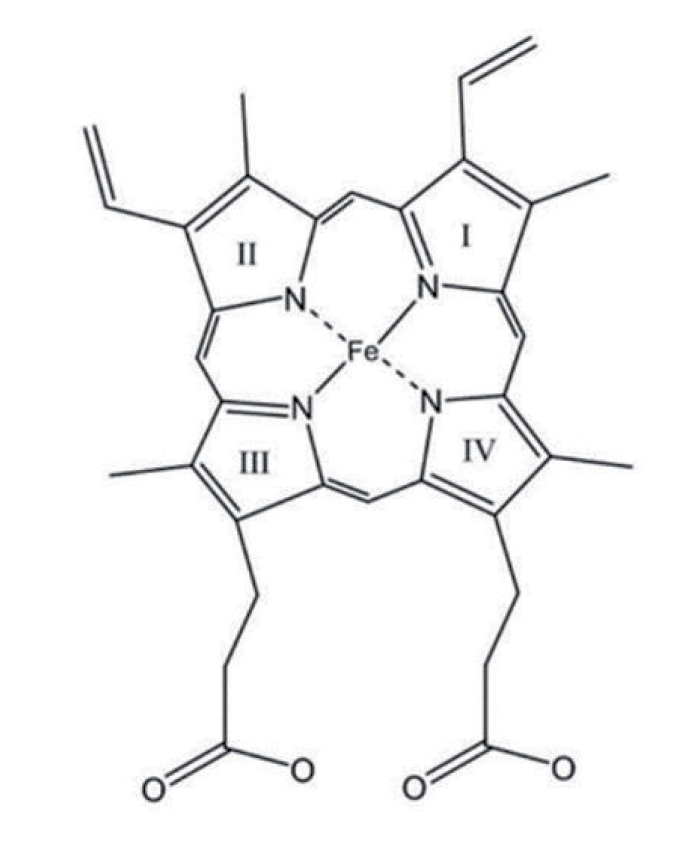
\includegraphics[width = 0.6\linewidth]{heme.png}% Here is how to import EPS art
	\caption{\label{fig:heme}Heme-b 분자구조}
\end{figure}
\begin{align}
	\begin{split}
		\ch{Enz(Por-Fe^{III}) + H_{2}O_{2}} \rightarrow \\
		\ch{Cpd I (Por^{+}-Fe^{IV} = O ) + H_{2}O} 
	\end{split}
\end{align}
\begin{align}
	\begin{split}
		\ch{Cpd I (Por^{+}-Fe^{IV} = O ) +  H_{2}O_{2}} \rightarrow \\
		\ch{Enz(Por-Fe^{III}) + H_{2}O + O_{2}}
	\end{split}
\end{align}
주변의 유기화합물중 질소와 같이 전기음성도가 큰 분자들은 과산화 수소의 수소와 화학결합을 하게 되고 과산화 수소는 $HO_{2}^{-}$상태가 될 것이다. 이때 enzyme의 철이온과 산소가 결합하게 된다. 이후에 다시 전기음성도가 큰 산소와 이전에 결합하였던 수소원자와 결합하게 되면서 $H_{2}O$가 생성되고 효소는 \ch{Cpd I (Por^{+}-Fe^{IV} = O )}와 같은 중간 생성물로 변환된다. \ch{Cpd I (Por^{+}-Fe^{IV} = O )}의 산소는 강한 음의 전하를 띠고 있어 주변의 과산화수소의 수소와 결합하게 된다. 과산화 수소의 2개의 수소가 모두 반응하게 되면 \ch{Cpd I (Por^{+}-Fe^{IV} = O )}의 산소는 $H_{2}O$, 그리고 남아 있는 산소는 $O_{2}$가 된다. 따라서 최종적인 화학 반응은 아래와 같아진다.

\begin{align}
	\ch{2 H_{2}O_{2}} \rightarrow \ch{2 H_{2}O + O_{2}}
\end{align}

위와 같은 촉매의 화학반응은 아래 식 (\ref{eq:first_ch}), (\ref{eq:second_ch})와 같이 단순화할 수 있다. 여기서 E는 촉매, S는 반응하는 물질이다.  
\begin{align}
	\ch{E + S} &\underset{k_{-1}}{\overset{k_{1}}{\longleftrightarrow}} \ch{ES} \label{eq:first_ch}\\
	\ch{ES} &{\overset{k_{2}}{\longrightarrow}} \ch{E + P} \label{eq:second_ch}
\end{align}

중간 생성물인 \ch{ES}의 농도가 일정한 steady state에 도달한 경우 식은 (\ref{eq:third_ch})와 같이 쓰여진다. 

\begin{align}
	\begin{split} \label{eq:third_ch}
		\frac{d[\ch{ES}]}{dt} & = 0 \\
	&= k_{1}[\ch{E}][\ch{S}] - k_{-1}[\ch{ES}] - k_{2}[\ch{ES}]
	\end{split}
\end{align}

이 때 식 (\ref{eq:forth_ch})가 성립한다.

\begin{align}\label{eq:forth_ch}
	[\ch{E}]_{0} = [\ch{E}] + [\ch{ES}]
\end{align}

위의식을 모두 정리하면 아래의 식이 성립한다.

\begin{align}
	K_{m} &= \frac{k_{-1} + k_{2}}{k_{1}}\\
	[\ch{ES}] &= \frac{[\ch{E}]_{0}[\ch{S}]}{[\ch{S}] + K_{m}}
\end{align}
따라서 \ch{P}의 생성 속도를 나타내는 식(Michaelis–Menten equation)은 아래와 같다.
\begin{align}
	\frac{d[\ch{P}]}{dt} &= k_{2}[\ch{ES}] = \frac{k_{2}[\ch{E}]_{0}[\ch{S}]}{[\ch{S}] + K_{m}}
\end{align}

역수를 취하면 아래의 라인웨버-버크 식(Lineweaver-Burk equation)을 얻게된다. 이를 통해 화학물의 농도, 촉매에 의한 반응속도의 관계를 확인할 수 있다. [2]

\begin{align}
	\frac{1}{v} &= \frac{1}{k_{2}[\ch{E}]_{0}} + \frac{K_{m}}{k_{2}[\ch{E}]_{0}[\ch{S}]}
\end{align}

본 실험에서는 감자 세포에 포함되어 있는 카탈레이즈에 의한 과산화수소 분해 속도 변화를 측정하고 이를 통해 Michaelis–Menten equation와 촉매에 대한 이해도를 높인다.

\section{\label{sec:level1}Experimental}
압력계, $250mL$ 삼각플라스크 일곱개, $30\%$ $H_{2}O_{2}$, 감자, 비커, 강판, 피펫, 열교환기, 얼음을 준비한다. $30\%$ 과산화수소를 7개의 삼각플라스크에 각각 $0.5\%$, $1\%$, $2\%$, $3\%$, $4\%$, $6\%$, $6\%$의 용액을 $30mL$를 준비한다. 이후에 감자즙을 천으로 짜서 추출액을 얻어 시험관에 넣고 ice bath에 보관한다. 이후에 과산화 수소가 들어 있는 삼각플라스크에 2mL의 추출액을 넣어 압력을 5초 간격으로 측정한다. 이후에 해당 추출액을 가열한 뒤 측정한 압력을 측정하여 control value로 활용한다. 단, 이 때 압력이 $200hPa$이 넘어가지 않도록 주의한다.

\section{\label{sec:level1}Reference}
[1] 김. (2010, August 1). 캐털레이스의 반응속도. In \textit{일반화학실험} (1th ed., p. 180).

[2] Oxtoby, D., Gillis, H., \& Campion, A. (2007, April 2). Rates of Chemical and Physical Processes. In \textit{Principles of Modern Chemistry} (6th ed., pp. pp.778-780). Cengage Learning.

[3] Garrett, R. H., \& Grisham, C. M. (2002, January 1). Proteins: Their Biological Functions and Primary Structure. In \textit{Principles of Biochemistry} (p. 120). Cengage Learning.

[4] Yuzugullu Karakus, Y. (2020, August 26). Typical Catalases: Function and Structure. \textit{Glutathione System and Oxidative Stress in Health and Disease}, 1–2. https://doi.org/10.5772/intechopen.90048


\end{document}
%
% ****** End of file apssamp.tex ******
